\documentclass[10pt,a4paper]{article}
\usepackage[utf8]{inputenc}
\usepackage{amsmath}
\usepackage{amsfonts}
\usepackage{amssymb}
\usepackage{indentfirst}
\usepackage{graphicx}
\author{José Miguel Leyva De la Cruz}
\title{Informe de Moogle!}
\date{}
\begin{document}
\maketitle

\section{Clase DataServer}
\setlength{\parindent}{1em} Esta clase tiene como principal objetivo crear un objeto de tipo \textbf{BBDD}, llamado \textbf{BaseDatos}, e inicializar la constante \textbf{Delimitors}, siendo esta un string que contiene todos los s\'imbolos de puntuaci\'on del idioma espa\~nol.

\setlength{\parindent}{1em} El objeto \textbf{BaseDatos} al ser de tipo \textbf{BBDD}, se encarga de crear la Base de Datos y el Universo de Palabras sobre el cual trabajar\'a el motor de b\'usqueda. Debido a lo costoso que es realizar semejante tarea, este objeto es creado antes de que la aplicaci\'on comience a funcionar, de esta manera se tendr\'a la base de datos lista para realizar todas las operaciones necesarias.

\section{Clase BBDD para crear la Base de Datos y el Universo de Palabras}
\begin{figure}[!h]
\centering
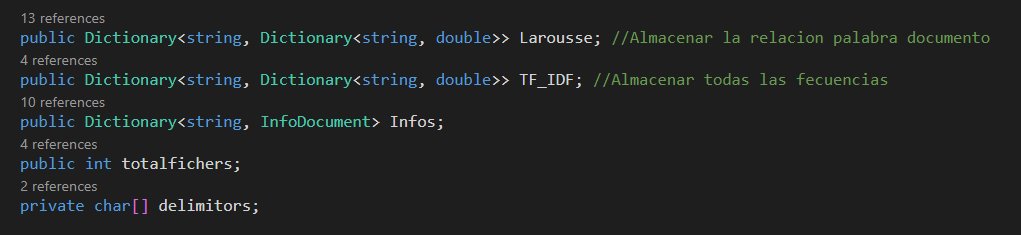
\includegraphics[width = 0.7\textwidth]{Clase BBDD.png}
\caption{Campos de la clase \textbf{BBDD}}
\end{figure}
\setlength{\parindent}{1em} La clase BBDD posee varios campos. Entre ellos se aprecian las tres estructuras m\'as importantes de la aplicaci\'on: \textbf{Larousse, TF\_IDF} e \textbf{Infos}. Su objetivo fundamental consiste crear un objeto en el cual, utilizando las estructuras antes mencionadas, almacena todo el universo de palabras que utilizar\'a el programa y les establece una relaci\'on con los documentos en los que se realizar\'a la b\'usqueda. Adem\'as, se encarga de la \textbf{Vectorizaci\'on} de los documentos. Todo este proceso ser\'a explicado a continuaci\'on.

\subsection{Larousse}
\setlength{\parindent}{1em} Esta estrucutura de datos es un diccionario encargado de almacenar en sus \textbf{keys} las palabras que se utilizar\'an para las operaciones de b\'usqueda, y en sus \textbf{values} son otro diccionario que guarda como \textbf{key}, los documentos en los que aparece dicha palabra y como \textbf{value}, la cantidad de veces que esta se repite en el texto del documento.

\subsection{TF\_IDF}
\setlength{\parindent}{1em} Muy parecida a \textbf{Larousse}, su \'unica diferencia es que en vez de almacenar la cantidad de veces que una palabra aparezca en un documento, guarda el valor de su \textbf{TF\_IDF} con respecto al documento en que se encuentra.

\subsection{\textbf{Infos}}
\setlength{\parindent}{1em} Este \'ultimo diccionario, tiene como \textbf{Keys}, las rutas de los documentos y como \textbf{values}, objetos del tipo \textbf{InfoDocument}, se aqbordar\'a sobre ellos m\'as adelante.

\subsection{Vectorizaci\'on}
\setlength{\parindent}{1em} Para realizar todas las operaciones de b\'usqueda y los diferentes c\'alculos que se abordar\'an en breve, la herramienta \textbf{Moogle!} utiliza un \textbf{Modelo Vectorial}. Para ello necesita expresar los documentos en forma de vectores. La vectorizaci\'on empleada consiste en que cada coordenada del vector es la cantidad de veces que una palabra se repite en un documento. Ejemplo: Suponga que existe un documento que posee $20$ palabras, una de estas palabras se repite $10$ veces, otra $7$ y la otra $3$, por tanto ese documento expresado en forma de vector ser\'ia $(10,7,3)$. Aqu\'i se aprecia la aplicaci\'on del diccionario \textbf{Larousse}, de esta manera se resume que los \textbf{values} del mismo son los documentos ya vectorizados.

\subsection{M\'etodo AddFile}
\setlength{\parindent}{1em} Este es el \'unico m\'etodo que posee la clase \textbf{BBDD}, recibe como par\'ametro un string (ficher) y tiene como funcionalidad, ``llenar'' el diccionario \textbf{Larousse}. Lo hace de la siguiente forma:\\

\setlength{\parindent}{1em} El constructor de la clase BBDD crea dentro de su \'ambito un array de string el cual contiene las rutas de todos los documentos, luego mediante el uso de un ciclo \textbf{for}, llama al m\'etodo \textbf{AddFile} en cada iteraci\'on del mismo, pas\'andole como argumento la direcci\'on de cada documento. Una vez dentro del m\'etodo, crea un string utilizando el m\'etodo ReadAllText de clase File y utiliza adem\'as el m\'etodo ToLower para leer todo el contenido del documento y normalizarlo a letras min\'usculas. Hecho esto crea un array de strings mediante el m\'etodo Split, utilizando el campo \textbf{Delimitors} de la clase \textbf{DataServer}. Ahora, itera por cada palabra utilizando un bucle \textbf{Foreach} y hace diferentes preguntas: Si la palabra no est\'a en \textbf{Larousse}, pues crea un diccionario nuevo cuyo par de \textbf{$<$Key,Value$>$} ser\'a el documento actual, y el n\'umero $1$, finalmente agrega la palabra y este nuevo diccionario al \textbf{Larousse}; si la palabra ya estaba guardada pero el documento es nuevo, le a\~nade a dicha palabra el nuevo documento; si la palabra ya estaba en \textbf{Larusse} y continua en el mismo documento, entonces aumentar en $1$, la cantidad de veces que dicha palabra aparece.
\setlength{\parindent}{1em} Ya vectorizados los documentos, se puede proceder al c\'alculo de la ``Norma'' de cada uno de ellos. La norma de un vector se calcula de la siguiente forma:

{\LARGE \begin{equation*}
\sqrt{\sum\limits_{i = 1}^{n} (x_i)^2}
\end{equation*}}
Siendo $x_i$ la componente i-\'esima del vector.

\setlength{\parindent}{1em} Una vez finalizado el proceso de Crear la Base de Datos y haber vectorizado los documentos. El constructor de la clase \textbf{BBDD} todo lo que le resta por hacer es inicializar \textbf{TF\_IDF}, mediante la clase \textbf{Frecuency}.

\section{Clase InfoDocument}
\setlength{\parindent}{1em} Esta clase, crea objetos de tipo \textbf{InfoDocument}, los cuales se utilizan para guardar las distintas propiedades de los documentos:
\begin{enumerate}
\item norma: Una vez vectorizado el documento, este valor almacena la norma del vector.
\item index: El \'indice del documento dentro del Diccionario \textbf{Infos}, de la clase \textbf{BBDD}.
\item cuerpo: El contenido del documento.
\end{enumerate}
\begin{figure}[!h] \label{fig:1}
\centering
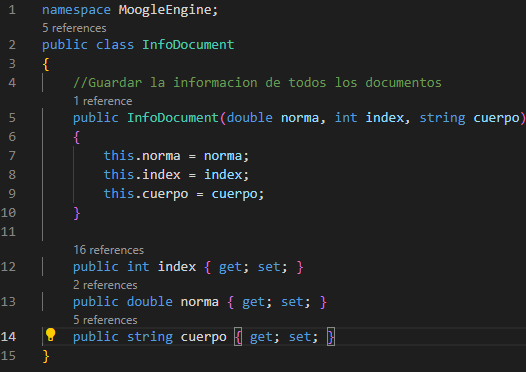
\includegraphics[width = 0.7\textwidth]{InfoDocument.png}
\caption{Clase \textbf{InfoDocument}}
\end{figure}

\section{Clase Frecuency, C\'alculo del TF\_IDF}
\subsection{M\'etodo TF\_IDF}
\setlength{\parindent}{1em} Este m\'etodo calcula el \textbf{TF\_IDF}, simplemente aplicando la f\'ormula, para la parte \textbf{TF} (Term Frecuency o Frecuencia de T\'erminos), dividie la cantidad de veces que una palabra aparece en un documento entre el total de t\'erminos que este posee. La parte \textbf{IDF} (Inverse Term Frecuency \'o Frecuencia Inversa) consiste en calcular el $\log_{10}$ del, total de documentos entre la cantidad de documentos en los que aparece el t\'ermino en cuesti\'on. Finalmente para obtener el \textbf{TF\_IDF} se multiplican ambas partes.
\begin{equation*}
TF.IDF = \frac{t_i}{d_j} * \log{\frac{N}{N_i}}
\end{equation*}
Siendo $t_i$, la cantidad de veces que aparece el i-\'esimo t\'ermino en el documento, $d_j$ la cantidad de t\'erminos que posee el documento, $N$ el total de documentos de la Base de Datos y $N_i$ la cantidad de documentos que contienen dicho t\'ermino.

\subsection{M\'etodo VectorWord}
\setlength{\parindent}{1em} Este m\'etodo recibe como par\'ametros un diccionario, \textbf{vector}, en el cual estar\'an todos los documentos que contienen el t\'ermino actual, y la cantidad de veces que se repite dicho t\'ermino; otro diccionario que contiene los documemtos y objetos de tipo \textbf{InfoDocument} y una variable que representa el total de ficheros. La funci\'on de este m\'etodo es iterar por todos los elementos de \textbf{vector}, convertir todo el contenido de cada elemento en un \textbf{array} de \textbf{string} mediante el m\'etodo \textbf{Split}, y luego llamar al m\'etodo \textbf{TF\_IDF} explicado anteriormente.

\subsection{M\'etodo GetTF\_IDF}
\setlength{\parindent}{1em} Este m\'etodo, recibe en sus par\'ametros el diccionario \textbf{Larousse} y el diccionario \textbf{Infos} ambos pertenecientes a la clase \textbf{BBDD}. Su funcionalidad consiste en iterar por cada una de las palabras almacenadas en el \textbf{Larousse}. Con cada iteraci\'on se llama al m\'etodo \textbf{VectoWord} y los resultados que este va obteniendo se guardan en un nuevo diccionario cuyas  \textbf{keys} son  palabras de \textbf{Larousse}, y sus \textbf{values} son otro diccionario que tiene como pares los documentos en los que aparece la palabra y el \textbf{TF\_IDF} de dicho archivo con respecto a la palabra.

\setlength{\parindent}{1em} Luego de todos estos procesos estar\'an creadas las tres estructuras fundamentales de la aplicaci\'on. Se puede notar que este procedimiento, es bastante largo y costoso para la pc, por tanto se realiza ante de arrancar el buscador; de esta forma, ya el programa tendr\'a todo su universo de palabras cargado, el \textbf{TF} de cada palabra con respecto a cada documento y el \textbf{IDF} de cada documento con respecto a cada palabra.
\begin{figure}[!h]
\centering
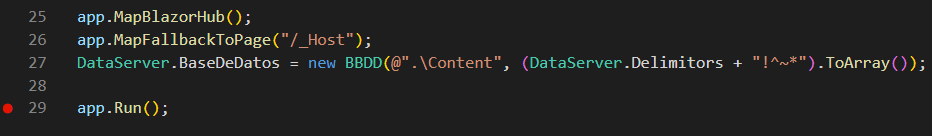
\includegraphics[width = 0.7\textwidth]{Comienzo de la APP.png}
\caption{\textbf{Crear la estructura el objeto BaseDatos antes de correr la aplicaci\'on}}
\end{figure}

\section{Clase Moogle}
\subsection{M\'etodo Scores}
\setlength{\parindent}{1em} Este m\'etodo como su nombre lo indica devuelve un array de double con los \textbf{Score} de cada documento con respecto a la b\'usqueda introducida por el usuario, dicho array es creado totalmente nuevo dentro del m\'etodo y tiene como tama\~no, la cantidad de documentos que haya en la base de datos. Recibe como par\'ametro una lista de palabras. Luego itera por cada una de las palabras de la lista, verifica si pertenecen al Universo de palabra creado y alamacenado en \textbf{Larousse}, en caso de que no: pues la "ignora", en caso contrario entonces: Indexa en la palabra en el Diccionario \textbf{TF\_IDF}, objeto BaseDeDatos creado anteriormente, e itera por cada documento que esta palabra tenga asociado (Recordar que estos diccionarios almacenaban el documento en el que aparece la palabra y el valor del TF\_IDF de dicho documento con respecto a la palabra). Utiliza el tipo de dato \textbf{var} para crear una variable "info", en la cual se guardar\'a el objeto \textbf{InfoDocument}, que le corresponde al documento sobre el cual se est\'e iterando. Finalmente en el array de nombre "score", se almacena en la posici\'on de info.Index la multiplicaci\'on de la cantidad de veces que la palabra aparece en la lista pasada como par\'ametro por el \textbf{TF\_IDF} del documento. 

\setlength{\parindent}{1em} Lo explicado anteriormente fue el producto escalar entre vectores, un vector \textbf{Query} y un vector \textbf{Document}, ambos vectorizados de la forma en que se explic\'o anteriormente. Luego de tener el producto escalar de ambos vectores, este n\'umero se divide entre el producto de las normas de cada vector. Haciendo esto se obtiene el valor del coseno del \'angulo que forman estos dos vectores, o sea todo este proceso fue aplicado para calcular el \textbf{Coseno de Similitud entre dos documentos con forma de vectores}, ya que mientras mayor sea el coseno, m\'as peque\~no ser\'a el \'angulo, es decir los vectores estar\'an m\'as ``cerca''. En otras palabras, es el documento que m\'as se ``parece'' a la b\'usqueda introducida, por tanto es el m\'as relevante. 

{\LARGE \begin{equation*}
\dfrac{V_1 * V_2}{|V_1| * |V_2|} = \cos \prec(V_1,V_2)
\end{equation*}}

\subsection{M\'etodo SnippetPlus}
\setlength{\parindent}{1em} Este m\'etodo utiliza 4 enteros: start (para identificar el indice en donde comenzar\'a el snippet), end (el indice del final del snippet), cant (cantidad de veces que una palabra de la query aparezca en el snippet que se analiza) y temp (para ir comparando). El snippet, no es m\'as que un fragmento del documento, pero no cualquiera, es el pedazo que mayor relevancia tenga con respecto a la b\'usqueda del usuario, es decir una vez obtenido el documento m\'as relevante, se extrae de el mismo el fragmento m\'as relevante. Este procedimiento consiste en iterar por las primeras 30 palabras del texto del documento, en caso de que posea menor cantidad que 30 palabras se devuelve el mismo documento, luego si existe una ocurrencia de alguna palabra de la query, se aumenta el n\'umero de la variable \textbf{cant}. Al finalizar este ciclo entonces comienza otro, que ocurrir\'a mientras la cantidad de palabras del documento menos start sea mayor o igual que 30. Entonces todo lo que hace es ``quitar'' la primera palabra y ``agregar'' una al final. Entonces se pregunta si: La palabra quitada est\'a en la b\'usqueda del usuario, entonces disminuye ``cant'', si la palabra agregada est\'a en la b\'usqueda entonces aumenta en $1$ la variable cant, luego se compara con ``temp'' y si es mayor entonces se actualizan los \'indices (start y end) y se le asigna a temp el valor de cant. Finalmente se tienen los \'indices de donde se encuentra el snippet de mayor importancia, se recorre el documento en el fragmetno que cae dentro de estos \'indices y se concatena cada palabra en un string, dicho string es el que se retorna al final del m\'etodo. 

\subsection{M\'etodo Evaluate}
\setlength{\parindent}{1em} Recibe entre sus par\'ametros el array de \textbf{scores} creado en el m\'etodo anterior y devuelve un array de objetos de tipo \textbf{SearchItem}. Este m\'etodo itera por cada uno de los documentos de \textbf{Infos}, llama al m\'etodo \textbf{Snippetplus} con cada documento, luego utilizando expresiones Lambda obtiene el t\'itulo de cada documento y finalmente crea un objeto \textbf{SearchItem} con este t\'itulo, el snippet y el score que est\'e guardado en la posici\'on que se\~nala la propiedad ``index'' del objeto \textbf{InfoDocument} en el que se est\'a iterando actualmente.
\end{document}